% !TEX root = ../main.tex

\section{Introduction}

Consider the traditional multi-party computational setting with a twist: Alice and Bob each have some data, they would like to know the output from running an agreed-upon function on their data, each does not want the other (or anyone else) to learn their data, and they want to simply submit their data (\eg encrypted) to a trustworthy system and come back later for the result. They are willing to pay for this service and understand that, in the worst case of massive collusion between the operators of this service (called trustees), their inputs may be exposed but the result will always be correct.

We assume the reader is familiar with blockchain technology, Ethereum, and smart contracts or decentralized apps (DApps). Can these technologies help? In theory? In practice? We seek to answer this question through direct experimentation. The abstract above builds the argument for why blockchain can help: (1) it provides a integral point of coordination where trustees can post and track progress on the evaluation; (2) it provides an in-band solution for paying the trustees (in either a cryptocurrency like ETH or in a stablecoin pegged to the value of governmental currency like the USD) in a way that is contingent on their performance; and (3) it can server as the public verifier and can reject any protocol proof that is not correct. When Alice and Bob retrieve the result (whether in plaintext or individually encrypted under their keys), they know it must be correct, otherwise it would not be there waiting for them.

Our experiments show that while in theory the idea is sound and we are able to successfully perform a secure function evaluation of a single logic gate (NAND gate) on Ethereum, the costs today are too prohibitive for it to be considered practical. We then turn to so-called layer-2 solutions and show that Arbitrum (an optimist roll-up that is based on the same trustee model we are already using~\cite{KGCWF18} can make Absentia substantially more practical (with room for further improvement).
 
\subsection{Key design decisions}

Note that we use the term secure function evaluation (SFE) to describe the stateless, one-shot evaluation that Absentia provides; and reserve the term multiparty computation (MPC) for a more setting where stateful computations might be performed over time.

\paragraph{Design decision: Trustee model.} In keeping with our priority for a submit-and-go protocol, someone has to perform the actual evaluation of the function on the inputs. We call these entities \emph{trustees}. We assume the number of trustees ($n$) can be chosen independently of the number of inputs. In Absentia, we simply our implementation to only support rubostness in the case that all trustees ($n$-out-of-$n$) participate, however this could modified to allow the protocol to proceed if only a threshold ($t$ out of $n$ for some $t<n/2$) of trustees participate (this, however, also reduces the number of trustees that need to collude to break the privacy, and potentially correctness, of the protocol).  

The remaining question is how can Alice and Bob find trustees they assume will not collude? We have several suggestions: (1) it could be based on personal connections; (2) perhaps commercial entities would emerge with either pre-established reputations or earn their reputation over time (similar to oracle providers) and through legally enforceable terms of service; or (3) trustees could be picked at random from a large set of trustees. While (3) may not sound convincing, it is essentially same threat model as the anonymous web-browsing tool Tor which is trusted by vulnerable users (perhaps Tor also uses flavours of (1) via its the EntryGuard program). 

\paragraph{Design decision: Ethereum.} While we are not the first to explore multi-party computation and its relationship to blockchain (see Section~\ref{sec:lit}), we believe we are the first to implement an MPC protocol on a public, commonly used blockchain; namely, Ethereum. The first research question we is whether MPC is even feasible on Ethereum, given the heavy cryptography it uses. Our paper establishes a benchmark that we hope to see improved through future research. Ethereum itself has scheduled scalability plans including Ethereum 2.0 (more transactions per second), and a lot of community resources are also being spent examining and implementing \emph{layer 2} solutions that move blockchain functionality off of the main chain without sacrificing many of its security benefits. Technologies include \emph{state channels}, \emph{sidechains}, and \emph{roll-ups}~\cite{GMR+20}. To experiment with these technologies, we also deploy and benchmark critical components of Absentia on Arbitrum~\cite{KGCWF18}, a recently proposed system for optimistic roll-ups (describe more in Section~\ref{sec:arb}). We now turn to another avenue for improvement, using state-of-the-art MPC protocols.

\paragraph{Design decision: Mix and match.} Starting with Yao in 1982~\cite{Yao82}, the question of how to securely evaluate a general function, when inputs are held by multiple people, has generated a rich body of literature in cryptography. In choosing an SFE/MPC protocol for the basis of Absentia, we looked for one with the following properties:

\begin{enumerate}
\item \textbf{Trustee model.} As justified above, we seek an MPC/SFE protocol that lets the input holders (\eg Alice and Bob) offload their inputs to a set of non-colluding trustees for evaluation. 
\item \textbf{Publicly verifiable} (aka publicly auditable or universally verifiable). Many MPC/SFE protocols are in the semi-honest (\ie honest-but-curious) model. Some are resilient to covert or malicious adversaries. We require that not only can adversarial behaviour  be detected by the participates in the protocol, but that it can be detected by anyone (\ie the public). This allows (a) Alice and Bob to offload the computational work to the trustees and still ensure the output is correct, even if they did not directly participate, and (b) Alice and Bob can go further and offload the verification itself to someone they trust---the Ethereum network in this case.
\item \textbf{Identifiable aborts.} If the protocol does not reach completion, anyone can establish which trustee aborted.
\item \textbf{Elliptic curve operations.} While Ethereum can in theory implement different types of cryptography (RSA groups, integer-based discrete logarithms groups, lattices, \etc), it has native support for its own cryptographic operations (ECDSA signatures) on the elliptic curve \texttt{secp256k1}. For easy of implementation, we prefer a SFE/MPC with the same cryptographic setting. 
\item \textbf{Circuit type.} When the function to be evaluated is represented as a circuit, the circuit could be based on logic gates (\ie NAND gates) or arithmatic operations (\eg additions and multiplications in a modular group). We are indifferent to this design parameter.
\end{enumerate}

One SPF protocol to meet our purposes is Mix and Match~\cite{JJ00} and we chose it based on our familiarity with it. We are also aware that the state-of-the-art MPC protocols are based on a different paradigm---based on \emph{Beaver triples}~\cite{beaver1997commodity}---initiated by the SPDZ protocol~\cite{damgaard2012multiparty,damgaard2013practical} with many followups (HighGear is a recent example~\cite{keller2018overdrive}). While SPDZ uses lattice-based somewhat homomorphic encryption (SME), this is during a pre-computation phase and Absentia (for now) assumes all pre-computation has been validated. SPDZ also appears amenable to a trustee model and one paper explores a publicly verifiable variant~\cite{baum2014publicly}, however since the authors do not compare themselves to Mix and Match, it would be a complete research project to determine if it is indeed faster. We note that it is not obviously categorically faster---for example, by not requiring public key operations at all: the publicly verifiable variant uses Pedersen commitments extensively.  

We are not aware of an explicit \emph{proof} that Mix and Match is publicly verifiable, however every step of the protocol is covered by a trustee issuing a non-interactive zero knowledge proof and it is later assumed to be by the authors in their auction application~\cite{JJ00}. Stated a different way, it appears that even when all trustees fully collude, trustees can only break privacy (and not integrity) with the exception of one sub-protocol, as noted by the authors~\cite{JJ00}, called the \emph{plaintext equality test} (PET). Despite the caveat, many have used the PET protocol as if it is publicly verifiable (some making justifications based on statistical arguments). Recently it was shown these statistical arguments are not sufficient, but the PET protocol can be made verifiable, even when \emph{all} trustees collude, with a simple additional check on the final output~\cite{mcmurtry2020test}.


\section{Preliminaries}

\subsection{Related work}
\label{sec:lit}

The blockchain literature has explored SFE and MPC in several regards. Perhaps the closest to Abstentia is Enigma~\cite{zyskind2015enigma} which offers stateful MPC as a service. The original academic proposal utilizes a custom blockchain. Now as a commercial project, the emphasis is on providing generic smart contracts with privacy. Engima runs on a Cosmos/Tendermint-based chain, which an Ethereum bridge contract that allows swapping crypto-assets. Abstentia is different in the following regards: (1) users provide the circuit they want evaluated, (2) Abstentia does not use trusted execution environments (TEE), and (3) we benchmark running natively on Ethereum. Like Enigma, Hawk also provides a privacy wrapper for contracts~\cite{kosba2016hawk}. It is based on succinct zero knowledge and fair MPC is described as an application of Hawk but not implemented.  

%HoneybadgerMPC~\cite{lu2019honeybadgermpc} uses a consensus algorithm to  ???

%~\cite{kiayias2016fair}

The literature has also explored moving computation off-chain while not losing privacy or correctness, however from the perspective a single entity's secret data (\ie verifiable computing as opposed to SFE/MPC). Examples include Zexe~\cite{bowe2020zexe}, ZkVM~\cite{zkvm}, and Raziel~\cite{sanchez2018raziel}. Another research direction, initiated by Andrychowicz \etal~\cite{andrychowicz2014secure}, explores how blockchain technologies can support an off-chain MPC to provide fairness. By contrast, Abstentia is performing the SFE on the blockchain. Closely related to SFE/MPC are zero knowledge proofs, whose uses in blockchain are now too prolific to adequately summerize here.

The blockchain literature has explored SFE and MPC in several regards. Enigma~\cite{zyskind2015enigma}, perhaps the closest to Absentia, offers stateful MPC as a service. The academic proposal was for its own blockchain and, now as a commercial project, the emphasis is more on providing generic smart contracts with privacy. While it does not run on Ethereum, a bridge contract is available to allow token transfers to their Cosmos/Tendermint-based chain. Absentia is different in the following regards: (1) users provide the circuit they want evaluated, (2) Absentia does not use trusted execution environments (TEE), and (3) we benchmark running natively on Ethereum. Like Enigma, Hawk also provides a privacy wrapper but is based on succinct zero knowledge~\cite{kosba2016hawk}. Fair MPC is described as an application of Hawk but not implemented.  


\subsection{Background}

We provide a basic overview of the Mix and Match protocol for secure function evaluation (SFE), while referring the reader to the original paper for the full details~\cite{JJ00}. Mix and Match uses a partially homomorphic encryption scheme; we instantiate it with the additive exponential Elgamal~\cite{CGS97}. We implement it over the elliptic curve \texttt{secp256k1} which is used natively by Ethereum (this results in gas savings).

\paragraph{Mix and Match: Pre-computation.} 

In a pre-computation stage, the following is tasks are completed. First, a set of $n$ trustees, identified by public keys, are chosen as well as a threshold of trustees needed to complete the protocol. We implement the simplest case: 2-out-of-2 (we call this distributed as opposed to threshold). Next, the trustees use a distributed key generation (DKG) protocol for creating $n$ shares of the decryption key, which can used for threshold $t-out-of-n$ decryption, as well as a single joint public key. Exponential Elgamal supports DKG and threshold decryption~\cite{Ped91a}.

In Mix and Match, a circuit of the function to be evaluated is produced using multi-input and multi-output lookup tables. We evaluate a single binary NAND gate (a universal gate that can create any circuit) which corresponds to a lookup table with two binary inputs (one from Alice and one from Bob) and a single binary output. During a pre-computation stage, the circuit for the function is established as a sequence of lookup tables (the output from one table can be used as an input to another). Each element of each lookup table is individually encrypted under the trustees' public key (we denote an encryption of $x$ as $\EncB{x}$). 

\begin{center}
\begin{tabular}{|c|c|c|}
  \hline
  A			& 	B			& 	Out   			\\ \hline
  $\EncB{0}$ 	&	$\EncB{0}$ 	& 	$\EncB{1}$ 	\\ \hline
  $\EncB{1}$ 	&	$\EncB{0}$ 	&  	$\EncB{1}$ 	\\ \hline
  $\EncB{0}$ 	&	$\EncB{1}$ 	& 	$\EncB{1}$ 	\\ \hline
  $\EncB{1}$ 	&	$\EncB{1}$ 	&  	$\EncB{0}$ 	\\ \hline
\end{tabular}
\end{center}

The encrypted table is then permuted row-wise. Each trustee mixes the rows, rerandomizes each ciphertext, and proves in zero knowledge that the result is correct. 

\begin{center}
\begin{tabular}{|c|c|c|}
  \hline
  A			& 	B			& 	Out   			\\ \hline
  $\EncB{0}$ 	&	$\EncB{1}$ 	& 	$\EncB{1}$ 	\\ \hline
  $\EncB{1}$ 	&	$\EncB{0}$ 	&  	$\EncB{1}$ 	\\ \hline
  $\EncB{1}$ 	&	$\EncB{1}$ 	&  	$\EncB{0}$ 	\\ \hline
  $\EncB{0}$ 	&	$\EncB{0}$ 	& 	$\EncB{1}$ 	\\ \hline
\end{tabular}
\end{center}

Complete circuits of such tables can be pre-computed by the trustees before Alice and Bob provide their inputs. Practically speaking, if sets of trustees were established, they could prepare circuits for commonly requested functions and post them publicly. When Alice and Bob decide to do an MPC, they can choose the pre-computed circuit (produced by a specific set of trustees). For the purposes of this paper, we assume circuits have been pre-computed and verified. In the future we may extend Abstentia to accept a circuit and complete set of proofs to verify its correct construction, but for this paper, we concentrate on building a verifier for the online phase.

\paragraph{Plaintext Equality Test (PET).} Let $\tuple{\EncB{a},\EncB{b}}$ denote two exponential Elgamal ciphertexts; encryptions of $a$ and $b$ respectively. The trustees will first compute $\EncB{z}=\EncB{a-b}$ using the additively homomorphic property. If the values are the same, $z=0$; otherwise $z\neq 0$. Each trustee will choose a random $r_i\neq0$, compute $\EncB{z_i}=\EncB{r_i*z_{i-1}}$ and prove correctness in zero knowledge. The resultant $\EncB{\hat{z}}=\EncB{\prod r_i*z}$ will still be $\EncB{0}$ when $a=b$ and will encrypt a randomly distributed non-zero integer otherwise. (The original proposal~\cite{JJ00} lets each trustee blind without using the result from the previous trustee---this adds asynchronicity but requires a critical security correction~\cite{mcmurtry2020test}). In the final step, the trustees decrypt and reveal $\hat{z}$.

\paragraph{Mix and Match: Online phase.} The trustees can begin with Alice's input $\EncB{a}$ and they compute a PET between $\EncB{a}$ and ciphertext in the column corresponding to Alice's input. They do the same for Bob. They locate the row that returns true for every input column. The output of this row can then be (1) transferred to the next gate, (2) decrypted publicly if it is a final output, or (3) proxy re-encrypted for Alice (and/or Bob) --- meaning it is obliviously and verifiably changed by the trustees from an encryption under the trustees' joint public key to an encryption under Alice's. For simplicity in Abstentia, we implement (2). We illustrate for the previous example and $a=1$ and $b=0$:

\begin{center}
\begin{tabular}{|c|c|c|}
  \hline
  A			& 	B			& 	Out   			\\ \hline
  $\mathsf{PET}(\EncB{a},\EncB{0}) = \mathtt{F}$ 	&	$\mathsf{PET}(\EncB{b},\EncB{1}) = \mathtt{F}$ 	& 	 	\\ \hline
  $\mathsf{PET}(\EncB{a},\EncB{1}) = \mathtt{T}$ 	&	$\mathsf{PET}(\EncB{b},\EncB{0}) = \mathtt{T}$ 	&  	$\EncB{1}$  	\\ \hline
  $\mathsf{PET}(\EncB{a},\EncB{1}) = \mathtt{T}$ 	&	$\mathsf{PET}(\EncB{b},\EncB{1}) = \mathtt{F}$ 	&  	 	\\ \hline
  $\mathsf{PET}(\EncB{a},\EncB{0}) = \mathtt{F}$ 	&	$\mathsf{PET}(\EncB{b},\EncB{0}) = \mathtt{T}$ 	& 	 	\\ \hline
\end{tabular}
\end{center}

Mix and Match.

* Mix-and-match~\cite{jakobsson2000mix}
Our system is based on mix-and-match protocol

a new approach to secure multiparty computation that does not heavily rely on verifiable secret sharing. 

It is based on creating a boolean representation of the computation to be done and representing it in a table. 

Private key is shared among the participants for working on the ciphertexts. 

The participants should decide on a function and its circuit representation before they proceed with the mix and match protocol.

Mix and match protocol guarantees that the participants only learn the output of their jointly chosen function and nothing else.






\section{Abstentia: system design}
\label{sec:system}

~\textbf{Alice:} can call loadFunds more than once. loadCiphertexts  x 4

~\textbf{Bob:} can call loadFunds more than once. loadCiphertexts x 4

~\textbf{Trustee1:} is also the manager. Trustee1 calls  
\begin{enumerate}
	\item loadOutputs  x 2
	\item  createRow1  x 4
\end{enumerate}
at the beginning of the protocol. 
\newline

The following is repeated for each PET (8 times): 
\begin{enumerate}
	\item PET\_subtract
	\item DHProve\_Trustee1Pf\_Rand
	\item DHProve\_Trustee1Pf\_PartialDec
	 \item FullDecryption
\end{enumerate}

After all PETs are run, Trustee1 has to run the following:
\begin{enumerate}
	\item matchingRow
	\item matchingValue
	\item createFinalDecryption
	\item loadFinalCiphertext
	\item DHProve\_Trustee1Pf\_PartialDec
	\item FullDecryption
\end{enumerate}

~\textbf{Trustee2:} 

The following is repeated for each PET (8 times): 
\begin{enumerate}
	\item DHProve\_Trustee2Pf\_Rand 
	\item DHProve\_Trustee2Pf\_PartialDec
\end{enumerate}
and calls DHProve\_Trustee2Pf\_PartialDec once for the final decryption.


\begin{table}[]
		\centering
	\begin{tabular}{|l|l|r|r|}
		\hline
		~\textbf{Contract} & ~\textbf{Function } & ~\textbf{Gas}  & ~\textbf{Gas Cost (\$)}  \\ \hline
		\multirow{9}{*}{}  
		& Load Funds & 28040  &1.50  \\ \cline{2-4} 
		& Check Balances &  30359& 1.63 \\  \cline{2-4} 
		&  Load Outputs&  300798 & 16.13 \\  \cline{2-4} 
		&  Create Row1 & 8741453 & 468.90 \\  \cline{2-4}
		Mixmatch.sol	&  matchingRow & 37547 &2.01  \\  \cline{2-4}
		& Find Matching Value &  40868&2.19 \\  \cline{2-4}
		&  Create Final Decryption&  4430611& 237.66 \\  \cline{2-4}
		& Send Excess Funds &  41110& 2.21 \\  \cline{2-4}
		& Withdraw Fund&  39221& 2.10 \\   \hline
		\multirow{8}{*}{} 
		&  Load Ciphertexts & 304668 & 16.34 \\  \cline{2-4}
		& Subtraction & 242131 & 12.99\\  \cline{2-4}
		&  T1 Randomization ZKP& 815340 &  43.74\\  \cline{2-4}
		PET.sol	&  T2 Randomization ZKP& 393561 &21.11  \\  \cline{2-4}
		& T1 Partial Dec ZKP& 364298 & 19.54\\  \cline{2-4}
		& T2 Partial Dec ZKP & 363612 & 19.50 \\  \cline{2-4}
		& Full Decryption  &  107086& 5.74 \\  \cline{2-4}
		&  Load Final Ciphertexts& 173945 & 9.33\\ \hline
	\end{tabular}
	\caption{Table description!! (Gas on Dec 01, 2020 is 0.000000087210450983 ETH)} \label{tab:gas}
\end{table}


\begin{table}[]
	\centering
	\begin{tabular}{|l|r|}
		\hline
		~\textbf{Code}	& ~\textbf{Size(bytes)}  \\ \hline
		bytecode	& 27178  \\ \hline
		deployed	& 26774  \\ \hline
		initialisation and constructor code 	& 404 \\ \hline
	\end{tabular}
	\caption{Code size}
\end{table}

\begin{table}[]
		\centering
	\begin{tabular}{|l|r|r|r|r|}
		\hline
		& ~\textbf{Alice} &  ~\textbf{Bob} & ~\textbf{Trustee1*}  & ~\textbf{Trustee2}  \\ \hline
		Number of Transactions	& 5 &5  &44  &17  \\ \hline
		Total gas cost	& 1246712 &  1246712& 52952603  & 6420996 \\ \hline
		Total cost in USD	&  66.87& 66.87 &2840.41  & 344.43 \\ \hline
	\end{tabular}
	\caption{Cost for each party} 
\end{table}

\begin{table}[]
		\centering
	\begin{tabular}{|l|r|}
	\hline
	~\textbf{Setting}	& ~\textbf{Total gas}  \\ \hline
	1 gate, 2 trustees	& 61867023  \\ \hline
	2 gate, 2 trustees	&  121240622 \\ \hline
	1 gate, 3 trustees	& 68288019 \\ \hline
\end{tabular}
	\caption{Different settings}
\end{table}


\begin{table}[]
		\centering
	\begin{tabular}{|l|r|r|r|r|r|r|r|}
		\hline
		&    \multicolumn{2}{c|}{~\textbf{Ethereum}} & \multicolumn{5}{c|}{~\textbf{Arbitrum}} \\ \hline
	   ~\textbf{Function}  &~\textbf{Tx} &~\textbf{Gas}   & ~\textbf{ L1} & ~\textbf{L1}  & ~\textbf{L2} &~\textbf{L2}& ~\textbf{Input Size} \\ 
	     & &  &~\textbf{Tx} &  ~\textbf{Gas} & ~\textbf{Tx}&~\textbf{arbgas}& ~\textbf{(bytes)} \\ 
		\hline
	    Deploy ec &  ~\href{https://kovan.etherscan.io/tx/0x088af056a640c1fe2188678e52484f89b7ba0bd9345bb0578d91c96aa480c59c}{Link}& 1103372& ~\href{https://kovan.etherscan.io/tx/0xa80f0eb0408f8f1c760abbc223b6a3b24780aba4b85f96ecbd6fb0dfe94bd606}{Link}&80152& ~\href{https://explorer.offchainlabs.com/#/tx/0x7c82717b52cb133c8855c0833d3cbf9ded19f884764fce78de3bb4e27feb63cd}{Link}&1304481&4978\\  \cline{1-8}
	  
	    Deploy PET &  ~\href{https://kovan.etherscan.io/tx/0xb76cda2c91907234afc0b971df893a6dbcdf83d482d2ff3d7d29b4a0b313002f}{Link}&5266352& ~\href{https://kovan.etherscan.io/tx/0x2ec73b92474c991d7b9f8ad1c46f95ef9125513897badb0c0c5faa19bd5b9a55}{Link}&386079& ~\href{https://explorer.offchainlabs.com/#/tx/0x2b1e63c81ca8ab7f4a6fe5333daab515a4e7408121771ae58e205ee037bceb50}{Link}&4260273&24172\\  \cline{1-8}
	
		Load Ciphertexts  & ~\href{https://kovan.etherscan.io/tx/0x2cb4bf0f6ce9fc7cabf0c152fdc61ccfff00a0f2e717c85da7eab806fa101b5b}{Link}&305309 &  \href{https://kovan.etherscan.io/tx/0x612e19481fff4ddd1c2dfe260908f15c7c74072a1e733597b4bab1c1209169f4}{Link}& 7869 &\href{https://explorer.offchainlabs.com/#/tx/0x28b3fa1a91d6d6e13005d352940861a026ac029fbc13a58dc969e98ffb5b392c}{Link} &  820507& 742\\  \cline{1-8}
	
		Subtraction & ~\href{https://kovan.etherscan.io/tx/0x6eeb3031c81af252df1fb806ae0a57643c20792df7336004465c6a74792c0016}{Link}&260729 & ~\href{https://kovan.etherscan.io/tx/0xa31a5653f3bfbdf7bcce4520c2a4f0e8d38fbc5c19036548199f805a4997cf68}{Link} & 5469& ~\href{https://explorer.offchainlabs.com/#/tx/0xbeff60af08f1b88deabe690322e26794d87595b332f1f1d01095a6a4528c4254}{Link} & 4789799& 550\\  \cline{1-8}
	
		T1 Randomization ZKP &~\href{https://kovan.etherscan.io/tx/0x30e8ccff5af6f3489ba2dc11e3198f0216487f380aa2a66ddf97e94650490e88}{Link} &819877 &  ~\href{https://kovan.etherscan.io/tx/0xc08cc82908b7e87e8ddc75695c4f29c3bce3d9a8caced144f003c59e23f4690e}{Link}&  11488&  ~\href{https://explorer.offchainlabs.com/#/tx/0xe3d1ba8bc653397dd67f3bfb602db0acce617668dc2ae2f30e038b4137a60e24}{Link}& 10972720& 644\\  \cline{1-8}
	
		  T2 Randomization ZKP & ~\href{https://kovan.etherscan.io/tx/0x6dd05a76c771089144583a685c2fb9a6b566a626aa86b568230faf83268fdd92}{Link}& 398245 & ~\href{https://kovan.etherscan.io/tx/0xd790b2edd8800a183068b3253d7e5b00e57d850bce8d9b8572494539b58c7e3c}{Link} &11440& ~\href{https://explorer.offchainlabs.com/#/tx/0x71535a6b6d0124cbd61a4993e5e831cc4ba151eec60b1c368a79686f3f5bc1f4}{Link} & 11069485 & 742 \\  \cline{1-8}
	
		 T1 Partial Dec ZKP &~\href{https://kovan.etherscan.io/tx/0x477b3e6b645cc672bbbe99ea3e7fa227962a3e1222071c266442a5ab8366e1bb}{Link} &366636 & ~\href{https://kovan.etherscan.io/tx/0xdd0ffc715dc5733bee36fd99d51898cf978de27ece76777099c4570929039a25}{Link} & 11452& ~\href{https://explorer.offchainlabs.com/#/tx/0x9f7fba14177790f6dad6ad9bb0ec3017803b466a27182768b11163162a3961c3}{Link} & 10692786& 742\\  \cline{1-8}

	 T2 Partial Dec ZKP &~\href{https://kovan.etherscan.io/tx/0x59a6282197cbd71b2c25cd5f3547b41ca7baf33322088f35273c97fce5cf8b56}{Link} &366089 & ~\href{https://kovan.etherscan.io/tx/0xb2a71505f192dd2119634ddd69070c52eb3a3d993aeb632ea8f823eb62f26e84}{Link} & 11512&  ~\href{https://explorer.offchainlabs.com/#/tx/0x724578f12940ebd653613c5037576540ce129ef277e4db67aff135711327e8f8}{Link} & 10689113& 742\\  \cline{1-8}
	
		Full Decryption & ~\href{https://kovan.etherscan.io/tx/0x172804db2abcef274dedfad8f31f84a0bb26c87826842589537f1d511402b282}{Link} & 124816 &  ~\href{https://kovan.etherscan.io/tx/0x10788165eacbbe25066c163fa0cf7a5af07da32c05af001d0f05ad8946974c6e}{Link}& 6236& ~\href{https://explorer.offchainlabs.com/#/tx/0x3515cc045805f2f9af9f378f4725ab4845679ca15ecd2e86758f8d53eb9a7353}{Link} & 4258675 & 422\\  \hline
	\end{tabular}
	\caption{Comparison with arbitrum (T1: Trustee1, T2: Trustee2)} 
\end{table}


\begin{figure}[h]
	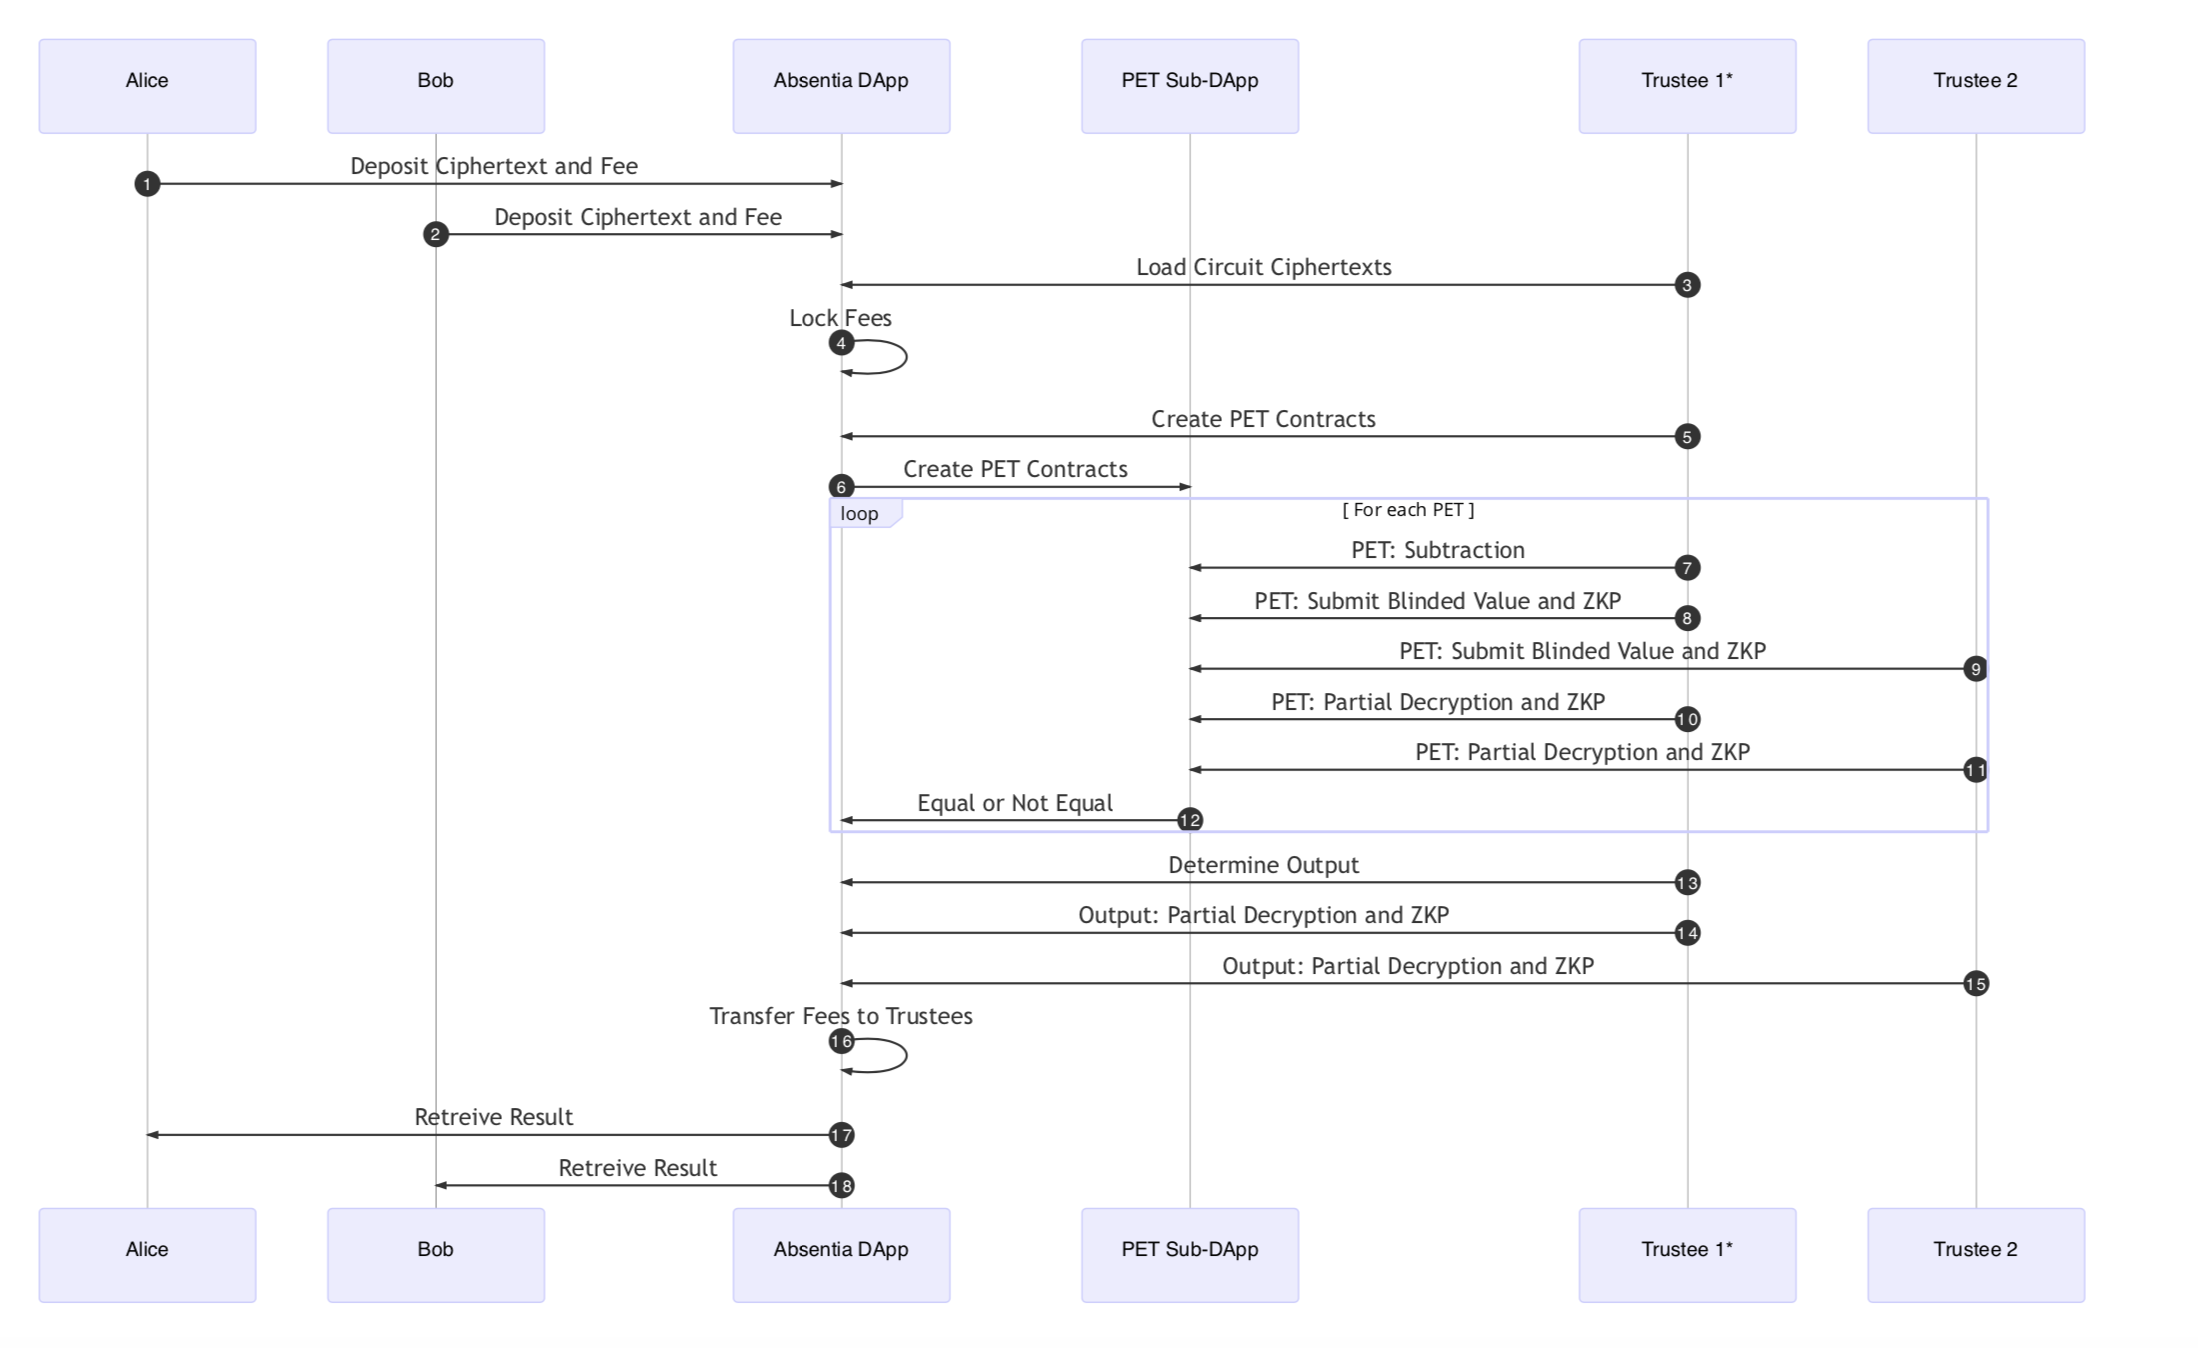
\includegraphics[width=15cm]{figures/diagram}
	\caption{figure}
	\centering
\end{figure}

%\begin{table}[]
%	\begin{tabular}{|l|l|l|l|l|l|}
%		\hline
%		  &  & ~\textbf{Ethereum} & \multicolumn{3}{c|}{~\textbf{Arbitrum}} \\ \hline
%		~\textbf{Contract} & ~\textbf{Function}  & ~\textbf{Gas}   &  ~\textbf{L1 Gas}  &~\textbf{L2 arbgas}& ~\textbf{Input Size (bytes)} \\ 
%		 \hline
%		\multirow{8}{*}{} 
%		&  loadCiphertexts & 304668 & 7869 & 820507& 832\\  \cline{2-6}
%		& PET\_subtract & 242131 & 5469& 4789799& 640\\  \cline{2-6}
%		&  DHProve\_Trustee1Pf\_Rand& 815340 &  11488& 10972720& 832\\  \cline{2-6}
%		PET.sol	&  DHProve\_Trustee2Pf\_Rand& 393561 &11440& 11069485 & 832 \\  \cline{2-6}
%		&  DHProve\_Trustee1Pf\_PartialDec& 364298 & 11452& 10692786& 832\\  \cline{2-6}
%		& DHProve\_Trustee2Pf\_PartialDec & 363612 & 11512& 10689113& 832\\  \cline{2-6}
%		& FullDecryption  &  107086& 6236& 4258675 & 512\\  \hline
%	\end{tabular}
%	\caption{Comparison with arbitrum} 
%\end{table}



Steps $2-6$ are repeated for each input cell.

Absentia is a system that performs secure function evaluation on Ethereum. The parties leave their secret, encrypted inputs to the system and the rest is handled in the absence of them (submit-and-go property).

The system is first implemented in Mathematica to have test vectors for the Solidity implementation. For our example, we used AND gate and there are two trustees that perform the computations. One of the trustees is designated as the manager who is responsible for creating and encrypting the table and finding the matching value at the end of the protocol.

The system is composed of two smart contracts and a library to perform elliptic curve operations.

The gas limit in Truffle is set to $0xBD6EE1$.

The elliptic curve library is taken from~\footnote{\url{https://github.com/orbs-network/elliptic-curve-solidity/blob/master/ECops.sol}}. As multiplication is the most expensive function, we do not perform the multiplication itself in the smart contract. Instead, we use the trick explained in~\footnote{\url{https://ethresear.ch/t/you-can-kinda-abuse-ecrecover-to-do-ecmul-in-secp256k1-today/2384}}. Multiplication is preformed off-chain and the function $ecmulVerify$ takes the multiplicand, scalar and the product as input and verifies that the multiplication is done correctly.

Contract size limit is 24KB according to EIP170. As our main contract is over this limit, we ran our test in Truffle by allowing unlimited contract size.

Factory design pattern is used to realize the system. Mix and match contract creates instances of PET contract for each cell in the NAND table , so that Alice and Bob's inputs are compared against related cells.

Depositing values to each PET vs depositing once

How payments are handled? 

Alice and Bob can deposit money any time they want during the protocol. They can also withdraw any excess amount from their balances as long as there is still enough funds left to pay the trustees. They can also withdraw funds either before the protocol starts or after the protocol ends, in the case where they accidentally deposited funds. Otherwise, the funds are kept for a month, until it can be withdrawn again. ~\footnote{\url{https://github.com/OpenZeppelin/openzeppelin-contracts/blob/master/contracts/utils/ReentrancyGuard.sol}} is used to prevent reentrancy attack.

Funds are transferred tot the trustees at the end of the protocol, after thay determined the final output. In another possible design, trustees can be paid at each step they performed towards reaching the final output.


\section{Design variant on layer 2 }
\label{sec:arb}

~\subsection{Arbitrum}
~\cite{kalodner2018arbitrum}
rollups on arbitrum

functions are performed off-chain and the result is written back to the chain, which is verifiable

dispute resolution



%\usetikzlibrary{calc}
%
%\resizebox{200pt}{200pt}{%
%
%	\begin{tikzpicture}
%	\coordinate (a) at (0,0);
%	\coordinate (b) at (0,1);
%	\coordinate (c) at (1,0);
%	\coordinate (d) at (1,1);
%	\coordinate (e) at (2,0);
%		\coordinate (f) at (2,1);
%	\draw (a) -- (b)node[pos=1.1,scale=0.25]{Client} 
%	(c) -- (d)node[pos=1.1,scale=0.25]{Server}
%	(e) -- (f)node[pos=1.1,scale=0.25]{Client} ;
%	\draw[-stealth] ($(a)!0.75!(b)$) -- node[above,scale=0.25,midway]{\href{https://www.google.ca/}{Text}}($(c)!0.75!(d)$);
%	\draw[stealth-] ($(a)!0.65!(b)$) -- node[below,scale=0.25,midway]{Hey} ($(c)!0.65!(d)$);
%	\end{tikzpicture}
%	}
%
%\begin{sequencediagram}
%	\newthread{t}{:Thread}
%	\newinst[1]{i}{:Instance}
%	
%	\begin{sdblock}{alt}{[condition]}
%		\begin{call}{t}{if\_true()}{i}{}
%		\end{call}
%		
%
%		
%		\begin{call}{t}{if\_false()}{i}{}
%		\end{call}
%	\end{sdblock}
%\end{sequencediagram}
%
%\begin{sequencediagram}
%\newthread[white]{u}{User}
%\newinst[3]{b}{Browser}
%\newinst[3]{t}{TPM}
%\newinst[3]{p}{TTP}
%
%\begin{call}{u}{Init()}{b}{}
%\end{call}
%
%\begin{call}{u}{\href{https://www.google.ca/}{Text}}{b}{}
%
%\mess{b}{verifyAIKAuthSecret}{t}
%
%\begin{call}{b}{get AIK$_{pub}$}{t}{AIK$_{pub}$}
%\end{call}
%
%\end{call}
%\begin{sdblock}{Loop}{}
%
%\begin{call}{u}{Do Something}{p}{AIK$_{pub}$}
%\end{call}
%\end{sdblock}
%\end{sequencediagram}


\begin{sequencediagram}
	\newthread{t}{:Thread}
	\newinst[1]{i}{:Instance}
	
	\begin{call}{t}{\href{https://kovan.etherscan.io/tx/0x10788165eacbbe25066c163fa0cf7a5af07da32c05af001d0f05ad8946974c6e}{Text}}{i}{return value}
	\end{call}
\end{sequencediagram}



\section{Discussion}

\begin{itemize}
\item Payments: fancier, contingent on who aborts, timeliness, \etc
\item Pre-comp: validate it , have pre-built and validated circuits, \etc
\item Implementation improvements: factory design and contract size
\item Proxy re-encryption instead of decryption
\item what else?
\end{itemize}